\documentclass[conference]{IEEEtran}
\IEEEoverridecommandlockouts
% The preceding line is only needed to identify funding in the first footnote. If that is unneeded, please comment it out.
\usepackage{cite}
\usepackage{amsmath,amssymb,amsfonts}
%\usepackage{algorithmic}
%TODO: Darf man das nutzen bei IEEE?
\usepackage{mathtools}
\usepackage{comment}
\usepackage{graphicx}
\usepackage{textcomp}
\usepackage{acronym}
\usepackage{url}
\usepackage{float}
\usepackage{amsmath}
\usepackage{diagbox}
\usepackage{amssymb}
\usepackage{enumitem}
\newcommand{\code}[1]{\texttt{#1}}
\usepackage[ruled,vlined,linesnumbered]{algorithm2e}

% custom macros used in algorithms
\newcommand{\var}[1]{#1}
\newcommand{\func}[1]{\texttt{#1}}

\usepackage{xcolor}
\usepackage[hidelinks]{hyperref} % load last
\Urlmuskip=0mu plus 1mu\relax
\def\UrlBreaks{\do\/\do-\do\_}
\def\BibTeX{{\rm B\kern-.05em{\sc i\kern-.025em b}\kern-.08em
    T\kern-.1667em\lower.7ex\hbox{E}\kern-.125emX}}


\pdfobjcompresslevel=0
\pdfminorversion=4
\hypersetup{pdfcreator={}, pdfproducer={}}
    
\begin{document}

\title{SOU: Towards Adaptive Offloading of Scientific Workflow Jobs
Across Multi-Cluster Environments}

\author{
    \IEEEauthorblockN{Niklas Fomin\IEEEauthorrefmark{1}, Jonathan Bader\IEEEauthorrefmark{1}, Leon Uwe Schaeffer\IEEEauthorrefmark{1}, Diellza Sherifi and Odej Kao}

    \IEEEauthorblockA{
        \{firstname.lastname\}@tu-berlin.de, Technische Universität Berlin, Germany\\
    }


}

%\IEEEpubid{\makebox[\columnwidth]{*equal contribution, alphabetical order \hfill} \hspace{\columnsep}\makebox[\columnwidth]{ }}

\maketitle

\begin{abstract}
Scientific workflows increasingly demand short turnaround times for scientific results, while complex analytical workloads can exceed the capacity of a single compute cluster.
Offloading jobs across multiple clusters can alleviate resource constraints and shorten execution time while controlling cost. 

This paper presents SOU, a middleware that offloads jobs across federated compute clusters. 

We propose an offloading heuristic based on a two-step prediction approach. First, a Bayesian regression model trained on historical executions predicts individual job runtimes. Second, a workflow simulation estimates the makespan of alternative offloading configurations, selecting jobs by predicted runtime or input data size until a user-defined time-to-result is met.

The method is implemented as an extension of the Snakemake workflow management system and is evaluated with two real-world bioinformatic workflows. 

In our evaluations, the proposed method meets the time-to-result target in five of six configurations and reduces cost by 40.1\% relative to a naive offloading baseline.

\end{abstract}

% from other papers
% Energy measurement, Supercomputers, Microprocessors, Multicore processing, Load modeling, High performance computing, Cluster computing, Power measurement, Software evaluation, Experimental comparison, DC power consumption, processor power, power model, multicore processor, processor workload analysis, processor power consumption estimation

% TODO: Refine
\begin{IEEEkeywords}
Distributed Computing, Job Offloading, Scientific Workflow, Cluster Computing, Machine Learning
\end{IEEEkeywords}

\section{Introduction} % 1/2 Seite
\label{sec:introduction}
Data-driven science produces massive datasets from high-throughput instruments, large simulations, and pervasive sensing~\cite{noauthororeditorfourth, liew_scientific_2017}. Scientific workflows are a key abstraction for structuring the resulting analyses~\cite{vivas_trends_2024}, and Scientific Workflow Management Systems (SWMSs) such as Snakemake~\cite{molder_sustainable_2021} and Nextflow~\cite{di_tommaso_nextflow_2017} let researchers define them in a modular and reproducible way. At scale, workflows comprise hundreds to thousands of jobs, run for hours to months, and demand substantial compute, storage, and networking resources~\cite{ahmad_scientific_2021, juve_characterizing_2013}, typically provided by large-scale infrastructures such as clusters or clouds~\cite{liu_survey_2015}.
%Scientific Workflow Management Systems (SWMSs) such as Snakemake~\cite{molder_sustainable_2021} and Nextflow~\cite{di_tommaso_nextflow_2017} let researchers define complex multi-step analyses in a modular and reproducible way.

%Because these workflows process large and complex datasets, they require substantial compute, storage, and networking resources \cite{ahmad_scientific_2021}. At scale, they may contain hundreds or thousands of jobs and run from hours to months \cite{juve_characterizing_2013, ferreira_da_silva_characterizing_2020}, typically relying on distributed infrastructures such as clusters, grids or clouds~\cite{liu_survey_2015, siar_offloading_2021}.

\begin{comment}
In heterogeneous compute environments, resources may be geographically and administratively distributed. Such settings introduce non-trivial scheduling and job allocation challenges, which have been addressed by numerous algorithms targeting different performance objectives \cite{shukla_fat-eto_2023,siar_offloading_2021,de_maio_multi-objective_2020,zhang_task_2017,wang_energy-efficient_2019,kaur_focalb_2021}. 
%A widely used approach, particularly in the cloud-continuum, is job offloading between available compute environments to satisfy user-defined objectives \cite{khan_fog_2017,mcc}.
\end{comment}

%Although workflow scheduling and resource allocation within single clusters have been extensively investigated, a single cluster can still be insufficient to satisfy the resource or time requirements of large-scale workflows.
Placing such jobs across distributed environments is a well-studied problem, and job offloading has become a common approach to meet user-defined objectives such as deadlines or energy budgets~\cite{siar_offloading_2021, shukla_fat-eto_2023, de_maio_multi-objective_2020, zhang_task_2017, wang_energy-efficient_2019}. Although scheduling within and across clusters has been studied extensively~\cite{hutchison_mip_2013}, a single cluster often remains insufficient for large-scale workflows: long-running workflows monopolize local resources and delay results.
Given that research institutions can often access federated computing resources such as shared HPC or the cloud beyond their on-premises infrastructure, scientists should be able to bundle these resources for accelerated time-to-result while maintaining control over operational expenditures, as every offloaded job incurs cost.

%Users often require faster turnaround times and may therefore rely on secondary resources to meet time constraints. In such cases, the systematic distribution of jobs to alternative clusters can alleviate resource contention and thereby improve overall workflow makespan.
%Motivated by this scenario, this work extends the concept of job offloading to the execution of scientific workflows in distributed multi-cluster environments \cite{hutchison_mip_2013}.



\begin{comment}
Fig.~\ref{fig:intro} illustrates the offloading scenario we consider in this paper. We assume a primary compute environment that serves as the default execution site, but may be unable to satisfy workflow deadlines due to limited resource capacity. To address this limitation, a secondary environment is available that can provide additional resources when necessary. 

All jobs are executed in the primary environment unless offloading is explicitly performed. A typical primary environment is an on-premise cluster that is readily accessible to users, provides limited computational capacity, and does not incur direct monetary cost. The secondary environment serves as an alternative execution site to which selected jobs can be offloaded. In practice, this secondary environment can correspond to an off-premise cluster with restricted capacity or to a cloud platform that offers resources on demand.

 As in many practical scenarios, particularly when using cloud resources, offloading introduces monetary costs proportional to the consumed resources and execution time. Therefore, the use of secondary environments must remain economically feasible, requiring careful control of offloading decisions. 
\end{comment}
%Our proposed lightweight method satisfies this requirement using the architecture depicted in Figure \ref{fig:intro}. We contribute a performance-aware placement middleware, implemented as an extension of Snakemake, that guides scientific workflow execution across multi-cluster environments.\footnote{{published after acceptance.}} 
Our proposed lightweight method satisfies this requirement using the architecture depicted in Fig.~\ref{fig:intro}. We contribute the Snakemake Offloading Utility (SOU), an offloading middleware implemented as an extension of Snakemake.\footnote{\url{https://git.tu-berlin.de/snakemake-offloader}} Given a user-defined time-to-result, SOU predicts job runtimes from historical executions, simulates the workflow makespan across clusters, and offloads jobs chosen by a pluggable criterion until the target is met, keeping the number of offloaded jobs, and thus cost, low.
%Our plugin accepts a user-specified, soft deadline for the workflow’s makespan and supports data-centric and performance-aware job placement strateiges that remain readily extensible.

\begin{comment}
The paper makes the following contributions:
\begin{enumerate}
  \item We propose a heuristic two-step approach: (i) predict job runtimes using linear models trained on historical data, and (ii) simulate workflow execution on multi-clusters using these predictions to select jobs for offloading that meet user-defined deadlines while minimizing cost.
  \item We provide our implementation as an extension to the Snakemake SWMS. The source code and the workflow execution data collected during our experiments are made publicly available.\footnote{{published after acceptance.}}
\end{enumerate}
\end{comment}



\section{Approach}
\label{sec:approach}
\begin{figure}[t]
\centering
\begin{tikzpicture}[
  font=\footnotesize, >={Stealth[length=1.5mm]},
  io/.style={draw, rounded corners=2pt, minimum width=3.9cm, minimum height=9mm, align=center},
  stp/.style={draw, rounded corners=1pt, fill=white, minimum width=2.45cm, minimum height=9mm, align=center},
  dot/.style={circle, fill=#1, inner sep=0pt, minimum size=1.6mm},
  job/.style={fill=#1, minimum size=1.7mm, inner sep=0pt}
]
% ---- inputs
\node[io, fill=red!10]  (wf)   at (2.0,4.4) {\hspace{9mm}Scientific workflow\\\hspace{9mm}+ time-to-result};
\node[io, fill=gray!10] (hist) at (6.6,4.4) {\hspace{7mm}Historical\\\hspace{7mm}executions};
% mini DAG icon
\begin{scope}[shift={(0.45,4.4)}]
  \node[dot=teal]   (a) at (0,0.22) {};
  \node[dot=violet] (b) at (-0.22,0) {}; \node[dot=teal] (c) at (0.22,0) {};
  \node[dot=orange] (d) at (0,-0.22) {};
  \draw (a)--(b) (a)--(c) (b)--(d) (c)--(d);
\end{scope}
% database icon
\begin{scope}[shift={(5.15,4.4)}]
  \draw[fill=white] (-0.2,0.2) -- (-0.2,-0.2) arc[start angle=180, end angle=360, x radius=0.2, y radius=0.07] -- (0.2,0.2);
  \draw[fill=white] (0,0.2) ellipse[x radius=0.2, y radius=0.07];
  \draw (-0.2,0) arc[start angle=180, end angle=360, x radius=0.2, y radius=0.07];
\end{scope}

% ---- SOU
\node[draw, rounded corners=2pt, fill=gray!4, minimum width=8.6cm, minimum height=21mm] (sou) at (4.3,2.45) {};
\node[anchor=north, font=\footnotesize\bfseries, inner sep=2pt] at (sou.north) {SOU};
\node[stp, fill=blue!8]                (pred) at (1.4,2.6)  {Runtime\\prediction};
\node[stp, fill=blue!8, very thick]    (sim)  at (4.3,2.6)  {Makespan\\simulation};
\node[stp, fill=orange!15, dashed]     (crit) at (7.2,2.6)  {Offloading criterion\\(pluggable)};
\draw[->] (pred) -- (sim);
\draw[->] (crit) -- (sim);
\draw[->] (sim.south) ++(0.35,0) arc[start angle=0, end angle=-180, x radius=0.35, y radius=0.2];
\node[font=\scriptsize\itshape, anchor=north, inner sep=1pt] at (4.3,1.93) {until time-to-result is met};

% ---- clusters
\node[io, fill=green!8] (c1) at (2.0,0.55) {\hspace{9mm}On-premises\\\hspace{9mm}cluster};
\node[io, fill=green!8] (c2) at (6.6,0.55) {\hspace{9mm}Shared HPC\\\hspace{9mm}or cloud};
\foreach \x/\y/\c in {0/0/teal,1/0/violet,2/0/teal,0/1/orange,1/1/teal,2/1/violet}
  \node[job=\c] at ($(0.3,0.45)+(\x*0.23,\y*0.23)$) {};
\foreach \x/\y/\c in {0/0/violet,1/0/teal,0/1/teal}
  \node[job=\c] at ($(4.9,0.45)+(\x*0.23,\y*0.23)$) {};

% ---- flow
\draw[->] (wf)   -- (wf |- sou.north);
\draw[->] (hist) -- (hist |- sou.north);
\draw[->] (c1 |- sou.south) -- node[font=\scriptsize\itshape, right] {local jobs} (c1);
\draw[->] (c2 |- sou.south) -- node[font=\scriptsize\itshape, right] {offloaded jobs} (c2);
\end{tikzpicture}
\caption{SOU overview: predicted job runtimes drive a makespan simulation in which a pluggable offloading criterion selects jobs for the secondary cluster until the user-defined time-to-result is met.}
\label{fig:intro}
\end{figure}


\paragraph{Workflow Makespan Prediction}
SOU operates by first predicting job runtimes from historical executions~\cite{bader_lotaru_2024, bader_sizey_2024, balis_evaluation_2023} to simulate the federated makespan prior to submission.
For each task, we collect the runtimes $\mathcal T$ of its historical jobs and their input size $x$. We define $x$ as the total size of the initial workflow inputs that a job and its ancestors consume, which we obtain by reconstructing the job DAG.
If $x$ and the runtime show a Pearson correlation of $\rho\geq0.8$, we fit a task-specific model with intercept $\beta_0$ and coefficient $\beta_1$, either by linear regression $t=\beta_0+\beta_1x$ or by Bayesian ridge regression $t\sim\mathcal N(\beta_0+\beta_1x,\sigma^2)$ to additionally capture uncertainty. Thus,
\[
\hat t_q(j)=
\begin{cases}
\mu_j+\Phi^{-1}(q)\,\sigma_j, & \rho\geq0.8,\\
\operatorname{median}(\mathcal T), & \text{otherwise}.
\end{cases}
\]
For the Bayesian model, $\mathcal N(\mu_j,\sigma_j^2)$ is the posterior predictive distribution, and quantiles $q>0.5$ give more conservative predictions that serve as a lever to meet the time-to-result with higher assurance~\cite{park_3sigma_2018}.

\paragraph{Heuristic Job Offloading Simulation}
% Algorithm
\begin{algorithm}[t]
\caption{Job Offloading via Makespan Prediction}
\label{alg:offloading}
\small
\SetKwFunction{Sim}{Simulate}
\SetKwProg{Fn}{Function}{:}{}
\KwIn{jobs $J$, target makespan $D$, criterion $\mathcal{C}$}
\KwOut{offloaded jobs $J_\mathrm{off}$}
$J_\mathrm{off}\gets\emptyset$\;
$(\hat M, J_\mathrm{def})\gets\Sim{$J, J_\mathrm{off}$}$\;
\While{$\hat M > D$ \textbf{and} $J_\mathrm{def}\setminus J_\mathrm{off}\neq\emptyset$}{
  add the first job of $J_\mathrm{def}\setminus J_\mathrm{off}$ selected by $\mathcal{C}$ to $J_\mathrm{off}$\;
  $(\hat M, J_\mathrm{def})\gets\Sim{$J, J_\mathrm{off}$}$\;
}
\Return the $J_\mathrm{off}$ with the lowest $\hat M$ found\;
\BlankLine
\Fn{\Sim{$J, J_\mathrm{off}$}}{
  $\hat M\gets 0$;\ $J_\mathrm{def}\gets\emptyset$\;
  \While{unfinished jobs in $J$}{
    \ForEach{ready job $j$}{
      $c\gets$ secondary \textbf{if} $j\in J_\mathrm{off}$ \textbf{else} primary\;
      \lIf{resources $\mathbf r(j)$ are free on $c$}{run $j$ on $c$ for $\hat t_(j)$}
      \lElse{defer $j$;\ $J_\mathrm{def}\gets J_\mathrm{def}\cup\{j\}$}
    }
    advance $\hat M$ to the next job completion\;
  }
  \Return $(\hat M, J_\mathrm{def})$\;
}
\end{algorithm}
SOU selects jobs for offloading by simulating the workflow execution~\cite{casanova_wrench_2020} with the predicted runtimes (Algorithm~\ref{alg:offloading}). It takes the jobs $J$, the time-to-result target $D$, and a selection criterion $\mathcal{C}$ and returns the set of jobs to offload, as a greedy alternative to searching all $2^{|J|}$ candidate sets.

Starting without offloading, it simulates the workflow once (lines 1--2). As long as the predicted makespan $\hat M$ exceeds $D$, it selects one more job by $\mathcal{C}$, adds it to $J_\mathrm{off}$, and re-simulates with this job on the secondary cluster (lines 3--5).
\emph{Longest Job First} (LJF) selects the job with the longest predicted runtime, as long-running jobs best amortize offloading overheads such as data transfer.
As illustrated in Figure~\ref{fig:approach}, LJF first offloads $j_2$ (30\,min), which lowers the predicted makespan from 73 to 43\,min. As this exceeds the 40\,min target, it offloads the next-longest job ($j_4$, 20\,min) and reaches 38\,min. \emph{Smallest Input Size First} (SISF) selects the job with the smallest input size $x$ and targets settings where offloading cost grows with data volume. Further criteria can be implemented.
In contrast, \emph{Primary Environment Fully Occupied} (PEFO) naively offloads whenever the primary cluster is saturated.

To predict the makespan of each selection, \code{Simulate} advances jobs by their predicted runtimes, running jobs in $J_\mathrm{off}$ on the secondary and all other jobs on the primary cluster (lines 11--12). A job whose resources $\mathbf r(j)$ are not free on its cluster waits and is recorded in $J_\mathrm{def}$ (line 13). The function returns $\hat M$ and $J_\mathrm{def}$ (line 15). Candidates for the next selection are those that had to wait for resources in the previous simulation, $J_\mathrm{def}\setminus J_\mathrm{off}$. Once $D$ is met or no candidate remains, SOU returns the configuration with the lowest predicted makespan (line 6).

\begin{figure}[t]
\centering
\begin{tikzpicture}[
  font=\footnotesize, >={Stealth[length=1.3mm]},
  job/.style={circle, draw=gray!70!black, fill=white, minimum size=5.2mm, inner sep=0pt, font=\tiny},
  off/.style={job, fill=orange!35, draw=orange!80!black},
  new/.style={off, very thick},
  edge/.style={->, gray!70, >={Stealth[length=0.9mm]}},
  nxt/.style={->, thick, gray!60!black}
]
% one snapshot: #1 x-centre, #2-#4 styles of the three middle jobs
\newcommand{\snapdag}[4]{%
  \begin{scope}[shift={(#1,1.45)}]
    \node[job] (s) at (0,0.75) {5};
    \node[#2]  (a) at (-0.62,0) {30};
    \node[#3]  (b) at (0,0) {12};
    \node[#4]  (c) at (0.62,0) {20};
    \node[job] (t) at (0,-0.75) {8};
    \foreach \m in {a,b,c} {\draw[edge] (s) -- (\m); \draw[edge] (\m) -- (t);}
  \end{scope}}
% makespan bar: #1 x-centre, #2 length, #3 colour, #4 label
\newcommand{\mkbar}[4]{%
  \begin{scope}[shift={({#1-1.1},0.2)}]
    \fill[#3] (0,-0.07) rectangle (#2,0.07);
    \draw[red!70!black, dashed, thick] (1.6,-0.17) -- (1.6,0.2);
    \node[font=\tiny, anchor=north west, inner sep=1pt] at (0,-0.08) {#4};
  \end{scope}}

% strategy strip
\node[draw, rounded corners=2pt, fill=gray!5, minimum width=8.6cm, minimum height=5.5mm] (strat) at (4.3,2.85) {};
\node[anchor=west, font=\scriptsize] at (strat.west) {\textbf{Offloading Criterion:}};
\node[draw=orange!80!black, fill=orange!20, rounded corners=1pt, font=\scriptsize, inner sep=1.5pt] (ljf) at (3.25,2.85) {LJF};
\node[font=\scriptsize, text=gray, anchor=west] at ($(ljf.east)+(0.05,0)$) {SISF $\mid$ PEFO};
\node[font=\scriptsize, anchor=east] at ($(strat.east)+(-0.1,0)$) {offloading order: 30 $\succ$ 20 $\succ$ 12};

\snapdag{1.25}{job}{job}{job}
\snapdag{4.3}{new}{job}{job}
\snapdag{7.35}{off}{job}{new}

\mkbar{1.25}{2.2}{red!45}{makespan 70 $>$ 50}
\mkbar{4.3}{1.75}{red!45}{makespan 55 $>$ 50}
\mkbar{7.35}{1.45}{teal!55}{makespan 45 $\le$ 50}

\foreach \x/\t in {1.25/start, 4.3/iteration 1, 7.35/iteration 2} \node[font=\tiny\itshape, text=gray!80!black] at (\x-0.95,2.3) {\t};
\draw[nxt] (2.2,1.45) -- node[font=\tiny, above] {offload} (3.35,1.45);
\draw[nxt] (5.25,1.45) -- node[font=\tiny, above] {offload} (6.4,1.45);

\node[font=\tiny, red!70!black, anchor=south, inner sep=1pt] at (1.75,0.4) {objective};
\node[font=\footnotesize, teal!70!black, anchor=west] at (7.92,0.2) {\ding{51}};
\end{tikzpicture}
\caption{Job selection: starting from a DAG annotated with predicted runtimes, the pluggable strategy (here LJF) offloads the next-ranked job and re-simulates the makespan until the objective (here time-to-result) is met.}
\label{fig:approach}
\end{figure}







\section{Evaluation}
\label{sec:evaluation}
\subsection{Experimental Setup}
\label{subsec:experimental-setup}

% Experiments
We evaluate our approach using two real-world bioinformatics workflows: \textit{rnaseq-star-deseq2}\footnote{\url{https://github.com/snakemake-workflows/rna-seq-star-deseq2}}, which aligns RNA sequencing reads and computes differential gene expression (135 jobs), and \textit{stained glass}\footnote{\url{https://github.com/mrvollger/StainedGlass}}, which computes sequence-identity heatmaps of genome assemblies (44 jobs). Per workflow, we run PEFO as baseline and LJF and SISF with two time-to-result targets each (310 and 250\,min for rnaseq-star-deseq2, 75 and 65\,min for stained glass).

Table~\ref{tab:results} reports the number of offloaded jobs $|J_\mathrm{off}|$, the prediction error (PE) of the predicted makespan relative to the observed median makespan, whether the time-to-result target was met, and the change in makespan and offloading cost relative to PEFO.
We derive costs from the runtime and the requested vCPUs, memory, and ephemeral storage of each offloaded job, priced at on-demand Google Kubernetes Engine (GKE) Autopilot rates\footnote{\url{https://cloud.google.com/kubernetes-engine/pricing}} as a reference for a commercial secondary environment.

% Infrastructure 
We use two Kubernetes clusters, each with two nodes (AMD EPYC 7282, 32 threads, 125 GiB RAM, 3.5 TB SSD), connected at 5 Gbit/s to emulate geo-distributed links.

\subsection{Experimental Results}
\label{subsec:experimental-results}
Makespan prediction with the Bayesian median ($q=0.5$) achieves a MAPE of 6.0\,\% for LJF and SISF and 6.4\,\% for PEFO. LJF deviates by at most 3.3\,\%, whereas SISF overestimates the makespan of rnaseq-star-deseq2 by 11.3\,\% and 17.4\,\%.
Overestimation is uncritical for the time-to-result, as both SISF runs still finish 35 and 37\,min early. Underestimation is not, as LJF with the 250\,min target of rnaseq-star-deseq2 misses it by 6\,min at a prediction error of only $-2.3$\,\%. All other experiments meet their target.
Offloading once the primary cluster runs out of resources (PEFO) shortens the makespan by 36.5\,\% for rnaseq-star-deseq2 and 31.0\,\% for stained glass, but also incurs the highest offloading cost. LJF and SISF trade part of this speed-up for cost and reduce the offloading cost by 40.6\,\% compared to PEFO at a 14.8\,\% longer makespan. For the 310\,min target of rnaseq-star-deseq2, LJF offloads only five jobs and lowers the cost from \$5.58 to \$2.07. Cost depends on the runtime and resources of the offloaded jobs rather than their number, as SISF with 35 jobs is cheaper than LJF with five for the 310\,min target. With the 250\,min target, SISF even outperforms PEFO in both makespan and cost.

\begin{figure}[t]
    \centering
    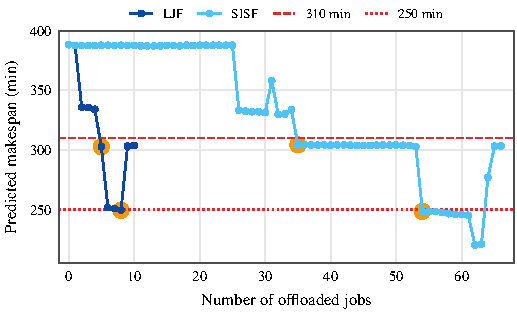
\includegraphics[width=\columnwidth]{img/evaluation/workflow_offloading_steps_rna-seq-star-deseq2.pdf}
    \caption{Bayesian predicted makespan after each offloading step for rnaseq-star-deseq2. Circles mark the job sets selected for each time-to-result target.}
    \label{fig:makespan-offloading-dependence}
\end{figure}

% Results Table
\begin{table}[t]
\caption{Makespan prediction error (PE) and change in median makespan ($\Delta$M) and offloading cost ($\Delta$C) relative to PEFO (\checkmark/$\times$: time-to-result met/missed).}
\label{tab:results}
\centering
\footnotesize
\setlength{\tabcolsep}{3pt}
\begin{tabular}{llrrrr}
\hline
\textbf{Workflow} & \textbf{Criterion ($C$)} & $|J_\mathrm{off}|$ & \textbf{PE} & $\Delta$\textbf{M} & $\Delta$\textbf{C} \\
\hline
rnaseq-star- & LJF (310\,min) \checkmark & 5 & +3.3\,\% & +29.8\,\% & $-$62.8\,\% \\
deseq2 & LJF (250\,min) $\times$ & 8 & $-$2.3\,\% & +12.7\,\% & $-$30.0\,\% \\
 & SISF (310\,min) \checkmark & 35 & +11.3\,\% & +21.2\,\% & $-$65.0\,\% \\
 & SISF (250\,min) \checkmark & 54 & +17.4\,\% & $-$6.3\,\% & $-$3.1\,\% \\
stained glass & LJF/SISF (75\,min) \checkmark & 2 & +1.1\,\% & +28.5\,\% & $-$70.4\,\% \\
 & LJF/SISF (65\,min) \checkmark & 6 & $-$0.8\,\% & +8.7\,\% & $-$20.4\,\% \\
\hline
\end{tabular}
\end{table}

% Makespan vs. Offloading
How many jobs are needed depends on the selection criterion, as Fig.~\ref{fig:makespan-offloading-dependence} shows for rnaseq-star-deseq2. Offloading the longest jobs first lowers the makespan right away, so LJF meets the 310\,min target after five jobs. SISF first offloads jobs with small inputs, so its prediction stays nearly constant from the second to the 25th job and it needs 26 jobs for the same target.

% Discussion
Our results show that simulating the makespan before execution lets SOU offload only as many jobs as a given time-to-result requires. Although most targets are met, the single miss occurs when the predicted makespan lies very close to the target. The time-to-result should therefore be understood as a soft constraint, as SOU selects a configuration that is predicted, but not guaranteed, to meet it. Moreover, offloading additional jobs does not always shorten the predicted makespan further (Fig.~\ref{fig:makespan-offloading-dependence}), which shows that the choice of jobs matters more than their number. 
Remaining prediction errors mainly stem from three sources. Runtimes vary under resource contention, tasks whose runtime does not correlate with input size fall back to the median runtime, and the simulation does not yet model job retries.

\section{Conclusion}
\label{sec:conclusion}
In this paper, we presented SOU, a Snakemake extension that offloads scientific workflow jobs across multi-cluster environments to meet user-defined deadlines.
SOU predicts job runtimes from historical executions and simulates DAG execution to estimate makespan and cost of alternative offloading configurations.
Our evaluation on real bioinformatics workflows shows that SOU meets makespan targets while reducing cost by 48.1\% compared to naive offloading.
Future work will incorporate online learning to re-evaluate offloading decisions at runtime~\cite{da_silva_online_2015, hilman_task_2018}, extend predictions to heterogeneous environments~\cite{bader_lotaru_2022, bader_lotaru_2024}, and consider network latency as well as energy and CO\textsubscript{2} metrics in the offloading criterion.


%\section*{Acknowledgments}
%\thanks{Funded by the Deutsche Forschungsgemeinschaft (DFG, German Research Foundation) as FONDA (Project 414984028, SFB 1404).}

% References from the full-paper introduction; replace with in-text \cite once the text is restored
\nocite{noauthororeditorfourth, liew_scientific_2017, vivas_trends_2024, molder_sustainable_2021, di_tommaso_nextflow_2017, ahmad_scientific_2021, juve_characterizing_2013, ferreira_da_silva_characterizing_2020, liu_survey_2015, siar_offloading_2021, shukla_fat-eto_2023, de_maio_multi-objective_2020, zhang_task_2017, wang_energy-efficient_2019, kaur_focalb_2021, khan_fog_2017, mcc, hutchison_mip_2013}

\bibliographystyle{IEEEtran}
\bibliography{bibliography}

\end{document}
